\documentclass[tikz]{standalone}
\usepackage{bm}
\usepackage{stix}

\definecolor{mplblue}{HTML}{1f77b4}
\definecolor{mplred}{HTML}{d62728}
\definecolor{mplpink}{HTML}{e377c2}

\def \layersep {2 cm}
\def \sitexsep {0.354 cm}
\def \siteysep {0.5 cm}
\def \sitezsep {0.354 cm}
\def \sitelen {5}
\def \convsize {1}

\def \sitenum {\the\numexpr \sitelen * \sitelen \relax}
\def \centerx {\the\numexpr \sitenum / 2 \relax}
\def \centeri {\the\numexpr \sitelen / 2 - 1 \relax}
\def \convmini {\the\numexpr \centeri - \convsize \relax}
\def \convmaxi {\the\numexpr \centeri + \convsize \relax}
\def \convminii {\the\numexpr \centeri - \convsize * 2 \relax}
\def \convmaxii {\the\numexpr \centeri + \convsize * 2 \relax}

\newcommand{\condeq}[4]{\ifnum#1=#2#3\else#4\fi}
\newcommand{\condlt}[4]{\ifnum#1<#2#3\else#4\fi}
\newcommand{\condgt}[4]{\ifnum#1>#2#3\else#4\fi}
\newcommand{\condle}[4]{\condgt{#1}{#2}{#4}{#3}}
\newcommand{\condge}[4]{\condlt{#1}{#2}{#4}{#3}}
\newcommand{\condconv}[5]{\condle{#1}{\centerx}{\condge{#2}{\convmini}{\condge{#3}{\convmini}{\condle{#3}{\convmaxi}{#4}{#5}}{#5}}{#5}}{#5}}
\newcommand{\condconvex}[5]{\condlt{#1}{\centerx}{\condge{#2}{\convmini}{\condge{#3}{\convmini}{\condle{#3}{\convmaxi}{#4}{#5}}{#5}}{#5}}{#5}}
\newcommand{\condconvI}[5]{\condlt{#1}{\centerx}{\condge{#2}{\convminii}{\condge{#3}{\convminii}{\condgt{\the\numexpr \sitelen - #2 - #3 \relax}{0}{#4}{#5}}{#5}}{#5}}{#5}}
\newcommand{\condconvH}[5]{\condle{#1}{\centerx}{\condge{#2}{\convminii}{\condge{#3}{\convminii}{\condgt{\the\numexpr \sitelen - #2 - #3 \relax}{0}{#4}{#5}}{#5}}{#5}}{#5}}

\tikzstyle{neuron}=[circle, draw]
\tikzstyle{annot}=[node distance=0.5 cm]

\pgfdeclarelayer{layer1}
\pgfdeclarelayer{arrow1}
\pgfdeclarelayer{layer2}
\pgfdeclarelayer{arrow2}
\pgfdeclarelayer{layer3}
\pgfdeclarelayer{arrow3}
\pgfdeclarelayer{layer4}
\pgfsetlayers{layer1,arrow1,layer2,arrow2,layer3,arrow3,layer4,main}

\begin{document}
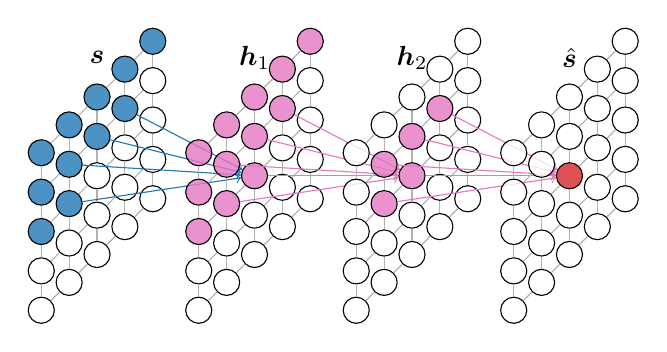
\begin{tikzpicture}

\begin{pgfonlayer}{layer1}
\foreach \x in {1, ..., \sitenum}
{
    \pgfmathtruncatemacro{\i}{(\x - 1) / \sitelen}
    \pgfmathtruncatemacro{\j}{\x - \i * \sitelen - 1}
    \node[neuron, fill=\condconvI{\x}{\i}{\j}{mplblue}{white}, fill opacity=0.8] (I\i\j) at (\j * \sitexsep, -\i * \siteysep + \j * \sitezsep) {};
}

\foreach \i in {0, ..., \the\numexpr \sitelen - 2 \relax}
    \foreach \j in {0, ..., \the\numexpr \sitelen - 1 \relax}
        \draw[black!30] (I\i\j) -- (I\the\numexpr \i + 1 \relax\j);

\foreach \i in {0, ..., \the\numexpr \sitelen - 1 \relax}
    \foreach \j in {0, ..., \the\numexpr \sitelen - 2 \relax}
        \draw[black!30] (I\i\j) -- (I\i\the\numexpr \j + 1 \relax);
\end{pgfonlayer}

\begin{pgfonlayer}{layer2}
\foreach \x in {1, ..., \sitenum}
{
    \pgfmathtruncatemacro{\i}{(\x - 1) / \sitelen}
    \pgfmathtruncatemacro{\j}{\x - \i * \sitelen - 1}
    \node[neuron, fill=\condconvH{\x}{\i}{\j}{mplpink}{white}, fill opacity=0.8] (H\i\j) at (\layersep + \j * \sitexsep, -\i * \siteysep + \j * \sitezsep) {};
}

\foreach \i in {0, ..., \the\numexpr \sitelen - 2 \relax}
    \foreach \j in {0, ..., \the\numexpr \sitelen - 1 \relax}
        \draw[black!30] (H\i\j) -- (H\the\numexpr \i + 1 \relax\j);

\foreach \i in {0, ..., \the\numexpr \sitelen - 1 \relax}
    \foreach \j in {0, ..., \the\numexpr \sitelen - 2 \relax}
        \draw[black!30] (H\i\j) -- (H\i\the\numexpr \j + 1 \relax);
\end{pgfonlayer}

\begin{pgfonlayer}{layer3}
\foreach \x in {1, ..., \sitenum}
{
    \pgfmathtruncatemacro{\i}{(\x - 1) / \sitelen}
    \pgfmathtruncatemacro{\j}{\x - \i * \sitelen - 1}
    \node[neuron, fill=\condconv{\x}{\i}{\j}{mplpink}{white}, fill opacity=0.8] (H2\i\j) at (2 * \layersep + \j * \sitexsep, -\i * \siteysep + \j * \sitezsep) {};
}

\foreach \i in {0, ..., \the\numexpr \sitelen - 2 \relax}
    \foreach \j in {0, ..., \the\numexpr \sitelen - 1 \relax}
        \draw[black!30] (H2\i\j) -- (H2\the\numexpr \i + 1 \relax\j);

\foreach \i in {0, ..., \the\numexpr \sitelen - 1 \relax}
    \foreach \j in {0, ..., \the\numexpr \sitelen - 2 \relax}
        \draw[black!30] (H2\i\j) -- (H2\i\the\numexpr \j + 1 \relax);
\end{pgfonlayer}

\begin{pgfonlayer}{layer4}
\foreach \x in {1, ..., \sitenum}
{
    \pgfmathtruncatemacro{\i}{(\x - 1) / \sitelen}
    \pgfmathtruncatemacro{\j}{\x - \i * \sitelen - 1}
    \node[neuron, fill=\condeq{\x}{\centerx}{mplred}{white}, fill opacity=0.8] (O\i\j) at (3 * \layersep + \j * \sitexsep, -\i * \siteysep + \j * \sitezsep) {};
}

\foreach \i in {0, ..., \the\numexpr \sitelen - 2 \relax}
    \foreach \j in {0, ..., \the\numexpr \sitelen - 1 \relax}
        \draw[black!30] (O\i\j) -- (O\the\numexpr \i + 1 \relax\j);

\foreach \i in {0, ..., \the\numexpr \sitelen - 1 \relax}
    \foreach \j in {0, ..., \the\numexpr \sitelen - 2 \relax}
        \draw[black!30] (O\i\j) -- (O\i\the\numexpr \j + 1 \relax);
\end{pgfonlayer}

\begin{pgfonlayer}{arrow1}
\foreach \x in {1, ..., \sitenum}
{
    \pgfmathtruncatemacro{\i}{(\x - 1) / \sitelen}
    \pgfmathtruncatemacro{\j}{\x - \i * \sitelen - 1}
    \condconvex{\x}{\i}{\j}{\draw[->, mplblue] (I\i\j) -- (H\centeri\centeri);}{}
}
\end{pgfonlayer}

\begin{pgfonlayer}{arrow2}
\foreach \x in {1, ..., \sitenum}
{
    \pgfmathtruncatemacro{\i}{(\x - 1) / \sitelen}
    \pgfmathtruncatemacro{\j}{\x - \i * \sitelen - 1}
    \condconv{\x}{\i}{\j}{\draw[->, mplpink] (H\i\j) -- (H2\centeri\centeri);}{}
}
\end{pgfonlayer}

\begin{pgfonlayer}{arrow3}
\foreach \x in {1, ..., \sitenum}
{
    \pgfmathtruncatemacro{\i}{(\x - 1) / \sitelen}
    \pgfmathtruncatemacro{\j}{\x - \i * \sitelen - 1}
    \condconv{\x}{\i}{\j}{\draw[->, mplpink] (H2\i\j) -- (O\centeri\centeri);}{}
}
\end{pgfonlayer}

\node[annot, above of=I02] {$\bm{s}$};
\node[annot, above of=H02] {$\bm{h}_1$};
\node[annot, above of=H202] {$\bm{h}_2$};
\node[annot, above of=O02] {$\hat{\bm{s}}$};

\end{tikzpicture}
\end{document}
